\documentclass[10pt, aspectratio=169, xcolor={svgnames}]{beamer}

% --- UTD Official Color Palette (Based on Official Branding) ---
\definecolor{utdorange}{RGB}{232,117,0}
\definecolor{utdgreen}{RGB}{18,71,52}
\definecolor{utdcyan}{RGB}{95,244,183}
\definecolor{utdcyangray}{RGB}{138,141,143}

% --- Packages ---
\usepackage[utf8]{inputenc}
\usepackage[T1]{fontenc}
\usepackage{graphicx}
\usepackage{tikz}
\usepackage{booktabs}
\usepackage{caption}
\usetikzlibrary{shadows, positioning}

% --- Beamer Theme & Branding Integration ---
\usetheme{Madrid}
\setbeamertemplate{navigation symbols}{}

% Standardize Colors for Beamer Elements (Blocks, Bullets, Titles)
\setbeamercolor*{structure}{fg=utdgreen}
\setbeamercolor*{palette primary}{fg=white, bg=utdgreen}
\setbeamercolor*{palette secondary}{fg=white, bg=utdorange}
\setbeamercolor*{palette tertiary}{fg=white, bg=utdgreen!80!black}
\setbeamercolor{titlelike}{parent=palette primary, fg=white, bg=utdorange}
\setbeamercolor{frametitle}{bg=utdorange, fg=white}
\setbeamercolor{block title}{bg=utdgreen, fg=white}
\setbeamercolor{block body}{bg=utdgreen!10, fg=black}

% Headline (Top Border) - Consistent with UTD Branding
\setbeamertemplate{headline}{
  \hbox{%
  \begin{beamercolorbox}[wd=0.3\paperwidth,ht=2.5ex,dp=1.125ex]{utdgreen}%
    {\color{utdgreen}\rule{\linewidth}{2.5ex}}
  \end{beamercolorbox}%
  \begin{beamercolorbox}[wd=0.7\paperwidth,ht=2.5ex,dp=1.125ex]{utdorange}%
    {\color{utdorange}\rule{\linewidth}{2.5ex}}
  \end{beamercolorbox}}
}

% Footline - Three-segment dynamic blocks
\setbeamertemplate{footline}{
  \leavevmode%
  \hbox{%
  \begin{beamercolorbox}[wd=.3333\paperwidth,ht=2.25ex,dp=1ex,center]{author in head/foot}%
    \usebeamerfont{author in head/foot} \color{white} Author Name (UTD)
  \end{beamercolorbox}%
  \begin{beamercolorbox}[wd=.3334\paperwidth,ht=2.25ex,dp=1ex,center]{title in head/foot}%
    \usebeamerfont{title in head/foot} \color{white} Short Title of Your Work
  \end{beamercolorbox}%
  \begin{beamercolorbox}[wd=.3333\paperwidth,ht=2.25ex,dp=1ex,right]{date in head/foot}%
    \usebeamerfont{date in head/foot} \color{white} \insertframenumber{} / \inserttotalframenumber\hspace*{2ex} 
  \end{beamercolorbox}}%
  \begin{tikzpicture}[remember picture, overlay]
    \fill[utdgreen] (current page.south west) rectangle ([xshift=0.3333\paperwidth, yshift=3.25ex]current page.south west);
    \fill[utdorange] ([xshift=0.3333\paperwidth]current page.south west) rectangle ([xshift=0.6667\paperwidth, yshift=3.25ex]current page.south west);
    \fill[black!80] ([xshift=0.6667\paperwidth]current page.south west) rectangle (current page.south east);
  \end{tikzpicture}
}

\begin{document}

% --- Slide 1: Refined Title Page (UTD Modern Professional) ---
\begin{frame}[plain]
    
\begin{tikzpicture}[remember picture, overlay]
        % Top bar: UTD Green and Orange accent
        \fill[utdgreen] (current page.north west) rectangle ([yshift=-1.2cm]current page.north east);
        \fill[utdorange] ([yshift=-1.2cm]current page.north west) rectangle ([yshift=-1.3cm]current page.north east);
        
        % UTD School Name
        \node[anchor=west, xshift=0.8cm, yshift=-0.6cm] at (current page.north west) {
            {\small \bfseries \color{white} THE UNIVERSITY OF TEXAS AT DALLAS} 
        };
        \node[anchor=east, xshift=-0.8cm, yshift=-0.6cm] at (current page.north east) {
            {\scriptsize \color{white} School of Economic, Political and Policy Sciences}
        };

        % Main Title Area
        \node[anchor=center, yshift=0.5cm] at (current page.center) {
            \begin{minipage}{0.9\paperwidth}
                \centering
                {\Huge \bfseries \color{utdgreen} Your Dissertation Title Here} \\[0.4cm]
                {\Large \color{utdorange} Subtitle or Specific Research Focus} \\[0.8cm]
                \textcolor{utdgreen}{\rule{0.6\textwidth}{1.2pt}} \\[0.8cm]
                {\large \scshape Dissertation Defense: Location or Context}
            \end{minipage}
        };

        % Presenter Info (Bottom Left)
        \node[anchor=south west, xshift=1cm, yshift=1.2cm] at (current page.south west) {
            \begin{tabular}{l}
                {\large \textbf{Author Name}} \\
                {\footnotesize Candidate for PhD in [Your Program]} \\
                {\footnotesize [Month Year]}
            \end{tabular}
        };

        % Committee Info (Bottom Right)
        \node[anchor=south east, xshift=-1cm, yshift=1.2cm] at (current page.south east) {
            \scriptsize
            \begin{tabular}{rl}
                \textbf{Dissertation Committee:} & \\
                \textcolor{utdgreen}{Professor A} & (Chair) \\
                Professor B & \\
                Professor C & \\
                Professor D &
            \end{tabular}
        };
        
        % Bottom subtle bar
        \fill[utdgreen] (current page.south west) rectangle ([yshift=0.3cm]current page.south east);
    \end{tikzpicture}
\end{frame}

% --- Slide 2: Roadmap (TOC) ---
\begin{frame}{Roadmap}
    \begin{columns}[t]
        \begin{column}{0.5\textwidth}
            \tableofcontents[sections={1-3}]
        \end{column}
        \begin{column}{0.5\textwidth}
            \tableofcontents[sections={4-6}]
        \end{column}
    \end{columns}
\end{frame}

\section{Introduction}

% --- Slide 3: Research Problem ---
\begin{frame}{Research Problem}
    \begin{itemize}
        \item \textbf{Timing as Investment}: Vaccination is an intertemporal health investment, not just a binary (Yes/No) choice.
        \item \textbf{The Cost of Delay}: Behavioral delay increases the cumulative attack rate by 5--10\% compared to supply-only scenarios.
        \item \textbf{Gap}: Standard models often ignore the \textit{shadow price of waiting} and how individuals discount future protection.
    \end{itemize}
    
    \begin{block}{Central Challenge}
        How to design time-consistent public health strategies that minimize the behavioral cost of waiting?
    \end{block}
\end{frame}

\section{Research Questions}

% --- Slide 4: Research Questions ---
\begin{frame}{Research Questions}
    \begin{enumerate}
        \item \textbf{Structural Parameterization}: What is the magnitude of the \textit{Behavioral Delay Multiplier} (BDM) in vaccination decisions?
        \item \textbf{Monetary Valuation}: What is the \textit{Shadow Price of Waiting} (RMB/month) for different vaccine attributes?
        \item \textbf{Policy Impact}: How do intertemporal preferences shape the Marginal Value of Public Funds (MVPF) for vaccination incentives?
    \end{enumerate}
\end{frame}

\section{Econometric Methodology}

% --- Slide 5: MNL and MXL Framework ---
\begin{frame}{MNL as Benchmark, MXL as Baseline}
    \begin{columns}[T]
        \begin{column}{0.48\textwidth}
            \setbeamercolor{block title}{bg=utdgreen, fg=white}
            \begin{block}{Multinomial Logit (MNL)}
                \small
                \begin{itemize}
                    \item Assumes \textbf{homogeneous} preferences across individuals
                    \item Coefficients are fixed
                    \item Simple and transparent benchmark
                    \item Imposes independence of irrelevant alternatives (IIA)
                \end{itemize}
            \end{block}
        \end{column}
        
        \begin{column}{0.48\textwidth}
            \setbeamercolor{block title}{bg=utdorange, fg=white}
            \begin{block}{Mixed Logit (MXL)}
                \small
                \begin{itemize}
                    \item Allows \textbf{random coefficients} (\textbf{preference heterogeneity})
                    \item Captures variation in time preferences across individuals
                    \item Relaxes IIA assumption
                    \item Estimated via simulated maximum likelihood
                \end{itemize}
            \end{block}
        \end{column}
    \end{columns}
    
    \vspace{0.8cm}
    \centering
    \textbf{Takeaway: Mixed logit is the preferred specification for capturing heterogeneity in vaccination timing preferences.}
\end{frame}

% --- Slide 6: Essay 1 Framework: Intertemporal Structural Modeling ---
\begin{frame}{Essay 1: Structural Parameterization of Time Preferences}
    \begin{itemize}
        \item \textbf{Objective}: Recover deep preference parameters ($\delta, \kappa$) using DCE data.
        \item \textbf{Structural Utility Function}:
            \[ U_{it} = \sum \beta X_{it} + \text{Discounting}(\tau) + \epsilon_{it} \]
        \item \textbf{Exponential vs. Hyperbolic}: 
            \begin{itemize}
                \item Exponential: $D(\tau) = \delta^\tau$
                \item Hyperbolic (quasi-): $D(\tau) = \kappa \delta^\tau$ for $\tau > 0$
            \end{itemize}
    \end{itemize}
    \begin{block}{The BDM Hypothesis}
        If $\kappa < 1$, individuals exhibit present bias, inflating the perceived cost of waiting.
    \end{block}
\end{frame}

% --- Slide 7: Essay 2 Framework: Monetary Valuation of Delay ---
\begin{frame}{Essay 2: Recovering the Shadow Price of Waiting}
    \begin{itemize}
        \item \textbf{MWTA}: Marginal Willingness to Accept compensation for a 1-unit increase in delay.
        \item \textbf{Estimation}: Ratio of the delay coefficient to the price coefficient.
            \[ MWTA_{\text{delay}} = - \frac{\partial U / \partial \text{Delay}}{\partial U / \partial \text{Price}} = - \frac{\beta_{\text{delay}}}{\beta_{\text{price}}} \]
        \item \textbf{Significance}: Converts abstract psychological time-cost into a standardized monetary metric for welfare analysis.
    \end{itemize}
\end{frame}

% --- Slide 8: Essay 3 Framework: Policy Impact & MVPF ---
\begin{frame}{Essay 3: Policy Impact \& MVPF}
    \begin{itemize}
        \item \textbf{MVPF}: Marginal Value of Public Funds for vaccination incentives.
        \item \textbf{Simulation}: Evaluates how time-inconsistent preferences $(\kappa < 1)$ distort the cost-effectiveness of public subsidies.
        \item \textbf{Key Question}: Can behavioral "nudges" or timing-based incentives achieve higher welfare gains than flat subsidies?
    \end{itemize}
    \begin{center}
        \textit{Goal: Optimize resource allocation by accounting for the behavioral delay multiplier.}
    \end{center}
\end{frame}

\section{Essay 1: Results and Discussion}

% --- Slide 9: Results I: Model Performance (Example Table) ---
\begin{frame}{Results I: Model Performance and Fit (Template Example)}
    \begin{itemize}
        \item \textbf{Comparison:} Comparison of Model A vs. Model B.
        \item \textbf{Statistical Superiority:} Model B significantly outperforms Model A.
        \item \textbf{Conclusion:} Your key takeaway regarding model fit.
    \end{itemize}
    \begin{table}
        \centering
        \small
        \begin{tabular}{lcc}
            \toprule
            Metric & Model A (Baseline) & Model B (Proposed) \\
            \midrule
            Log-Likelihood & -X,XXX.XXX & \textbf{-X,XXX.XXX} \\
            AIC & XX,XXX.XXX & \textbf{XX,XXX.XXX} \\
            Obs. (N $\times$ T) & X,XXX & X,XXX \\
            \bottomrule
        \end{tabular}
    \end{table}
\end{frame}

% --- Slide 10: Present Bias Visualization ---
\begin{frame}{Present Bias Visualization}
    \centering
    \vspace{0.2cm}
    \small Individuals disproportionately discount short delays relative to longer delays.
    
    \vfill
    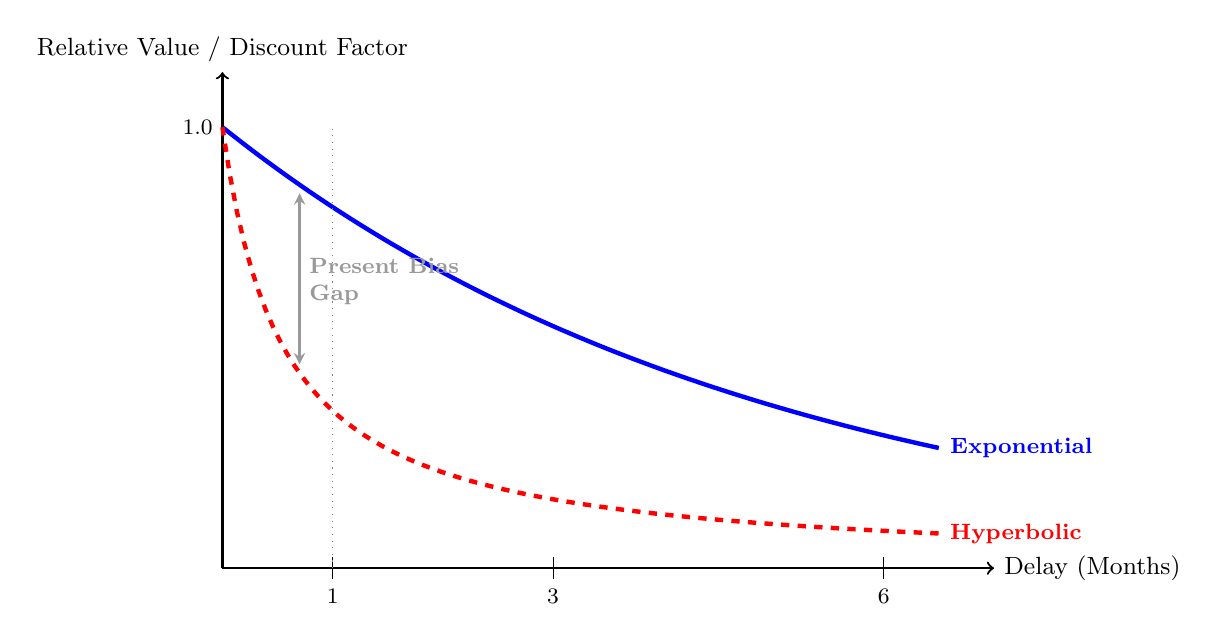
\begin{tikzpicture}[scale=1.4]
        % Axes
        \draw[->, thick] (0,0) -- (7,0) node[right] {\small Delay (Months)};
        \draw[->, thick] (0,0) -- (0,4.5) node[above] {\small Relative Value / Discount Factor};
        
        % Ticks
        \draw (0,4) node[left] {\footnotesize 1.0};
        \foreach \x in {1,3,6}
            \draw (\x,0.1) -- (\x,-0.1) node[below] {\footnotesize \x};
        
        % Exponential Curve (Blue, Smooth/Gradual)
        \draw[blue, ultra thick, domain=0:6.5, samples=100] plot (\x, {4*exp(-0.2*\x)}) 
            node[right] {\footnotesize \textbf{Exponential}};
        
        % Hyperbolic Curve (Red, Steeper drop)
        \draw[red, ultra thick, dashed, domain=0:6.5, samples=100] plot (\x, {4/(1 + 1.8*\x)}) 
            node[right] {\footnotesize \textbf{Hyperbolic}};
            
        % Annotation: Present Bias Gap
        \draw[<->, >=stealth, thick, gray!80] (0.7, 1.85) -- (0.7, 3.4);
        \node[right, gray!80, align=left] at (0.7, 2.6) {\footnotesize \textbf{Present Bias}\\[-0.5ex] \footnotesize \textbf{Gap}};
        
        % Highlighting the early steepness
        \draw[gray, dotted] (1, 0) -- (1, 4);
    \end{tikzpicture}
    \vfill
\end{frame}

% --- Slide 11: Results II: Quantifying Key Parameters ---
\begin{frame}{Results II: Quantifying Key Parameters}
    \begin{columns}[T]
        \column{0.5\textwidth}
        \begin{block}{Parameter Estimates}
            \begin{itemize}
                \item $\hat{\alpha} = 0.XXX$ (Description)
                \item $\hat{\beta} = 0.XXX$ (Description)
            \end{itemize}
        \end{block}
        \column{0.5\textwidth}
        \begin{alertblock}{Interpretation}
            \begin{itemize}
                \item Discuss the significance of the results.
                \item Relate back to your core hypothesis.
            \end{itemize}
        \end{alertblock}
    \end{columns}
    \centering
    \vspace{0.5cm}
    \textit{Conclusion: A concise summary of what these numbers imply for your theory.}
\end{frame}

% --- Slide 12: Results III: The BDM ---
\begin{frame}{Results III: The Behavioral Delay Multiplier (BDM)}
    \begin{itemize}
        \item \textbf{Concept:} Ratio of \textit{perceived} to \textit{objective} waiting time.
        \item \textbf{Calculation:} $BDM = \frac{1}{1 - \hat{\kappa}} = \frac{1}{1 - 0.225} \approx \mathbf{1.29}$.
        \item \textbf{Interpretation:} A delay is experienced as \textbf{29\% longer} than its objective duration.
        \item \textbf{Example:} A 30-day delay is perceived as approximately \textbf{38.7 days}.
    \end{itemize}
    \begin{center}
        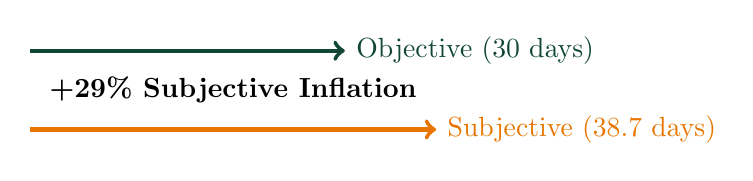
\begin{tikzpicture}
            \draw[->, ultra thick, utdgreen] (0,0) -- (4,0) node[right] {Objective (30 days)};
            \draw[->, ultra thick, utdorange] (0,-1) -- (5.16,-1) node[right] {Subjective (38.7 days)};
            \node at (2.58,-0.5) {\textbf{+29\% Subjective Inflation}};
        \end{tikzpicture}
    \end{center}
\end{frame}

% --- Slide 13: Results IV: Trust as a Behavioral Stabilizer ---
\begin{frame}{Results IV: MWTA by Institutional Trust}
    \begin{columns}[T]
        \begin{column}{0.6\textwidth}
            \begin{itemize}
                \item \textbf{Heterogeneity:} Institutional trust significantly moderates the shadow price of waiting.
                \item \textbf{High Trust Group:} MWTA = \textbf{32.4 RMB/month} (Highest patience).
                \item \textbf{Low Trust Group:} MWTA = \textbf{37.1 RMB/month}.
                \item \textbf{Neutral Group:} MWTA = \textbf{75.6 RMB/month} (Highest sensitivity/impatience).
            \end{itemize}
            \begin{block}{Key Finding}
                Trust acts as a "behavioral stabilizer." Individuals with neutral trust levels are the most sensitive to delays, requiring over \textbf{double} the compensation compared to high-trust individuals.
            \end{block}
        \end{column}
        \begin{column}{0.4\textwidth}
            \centering
            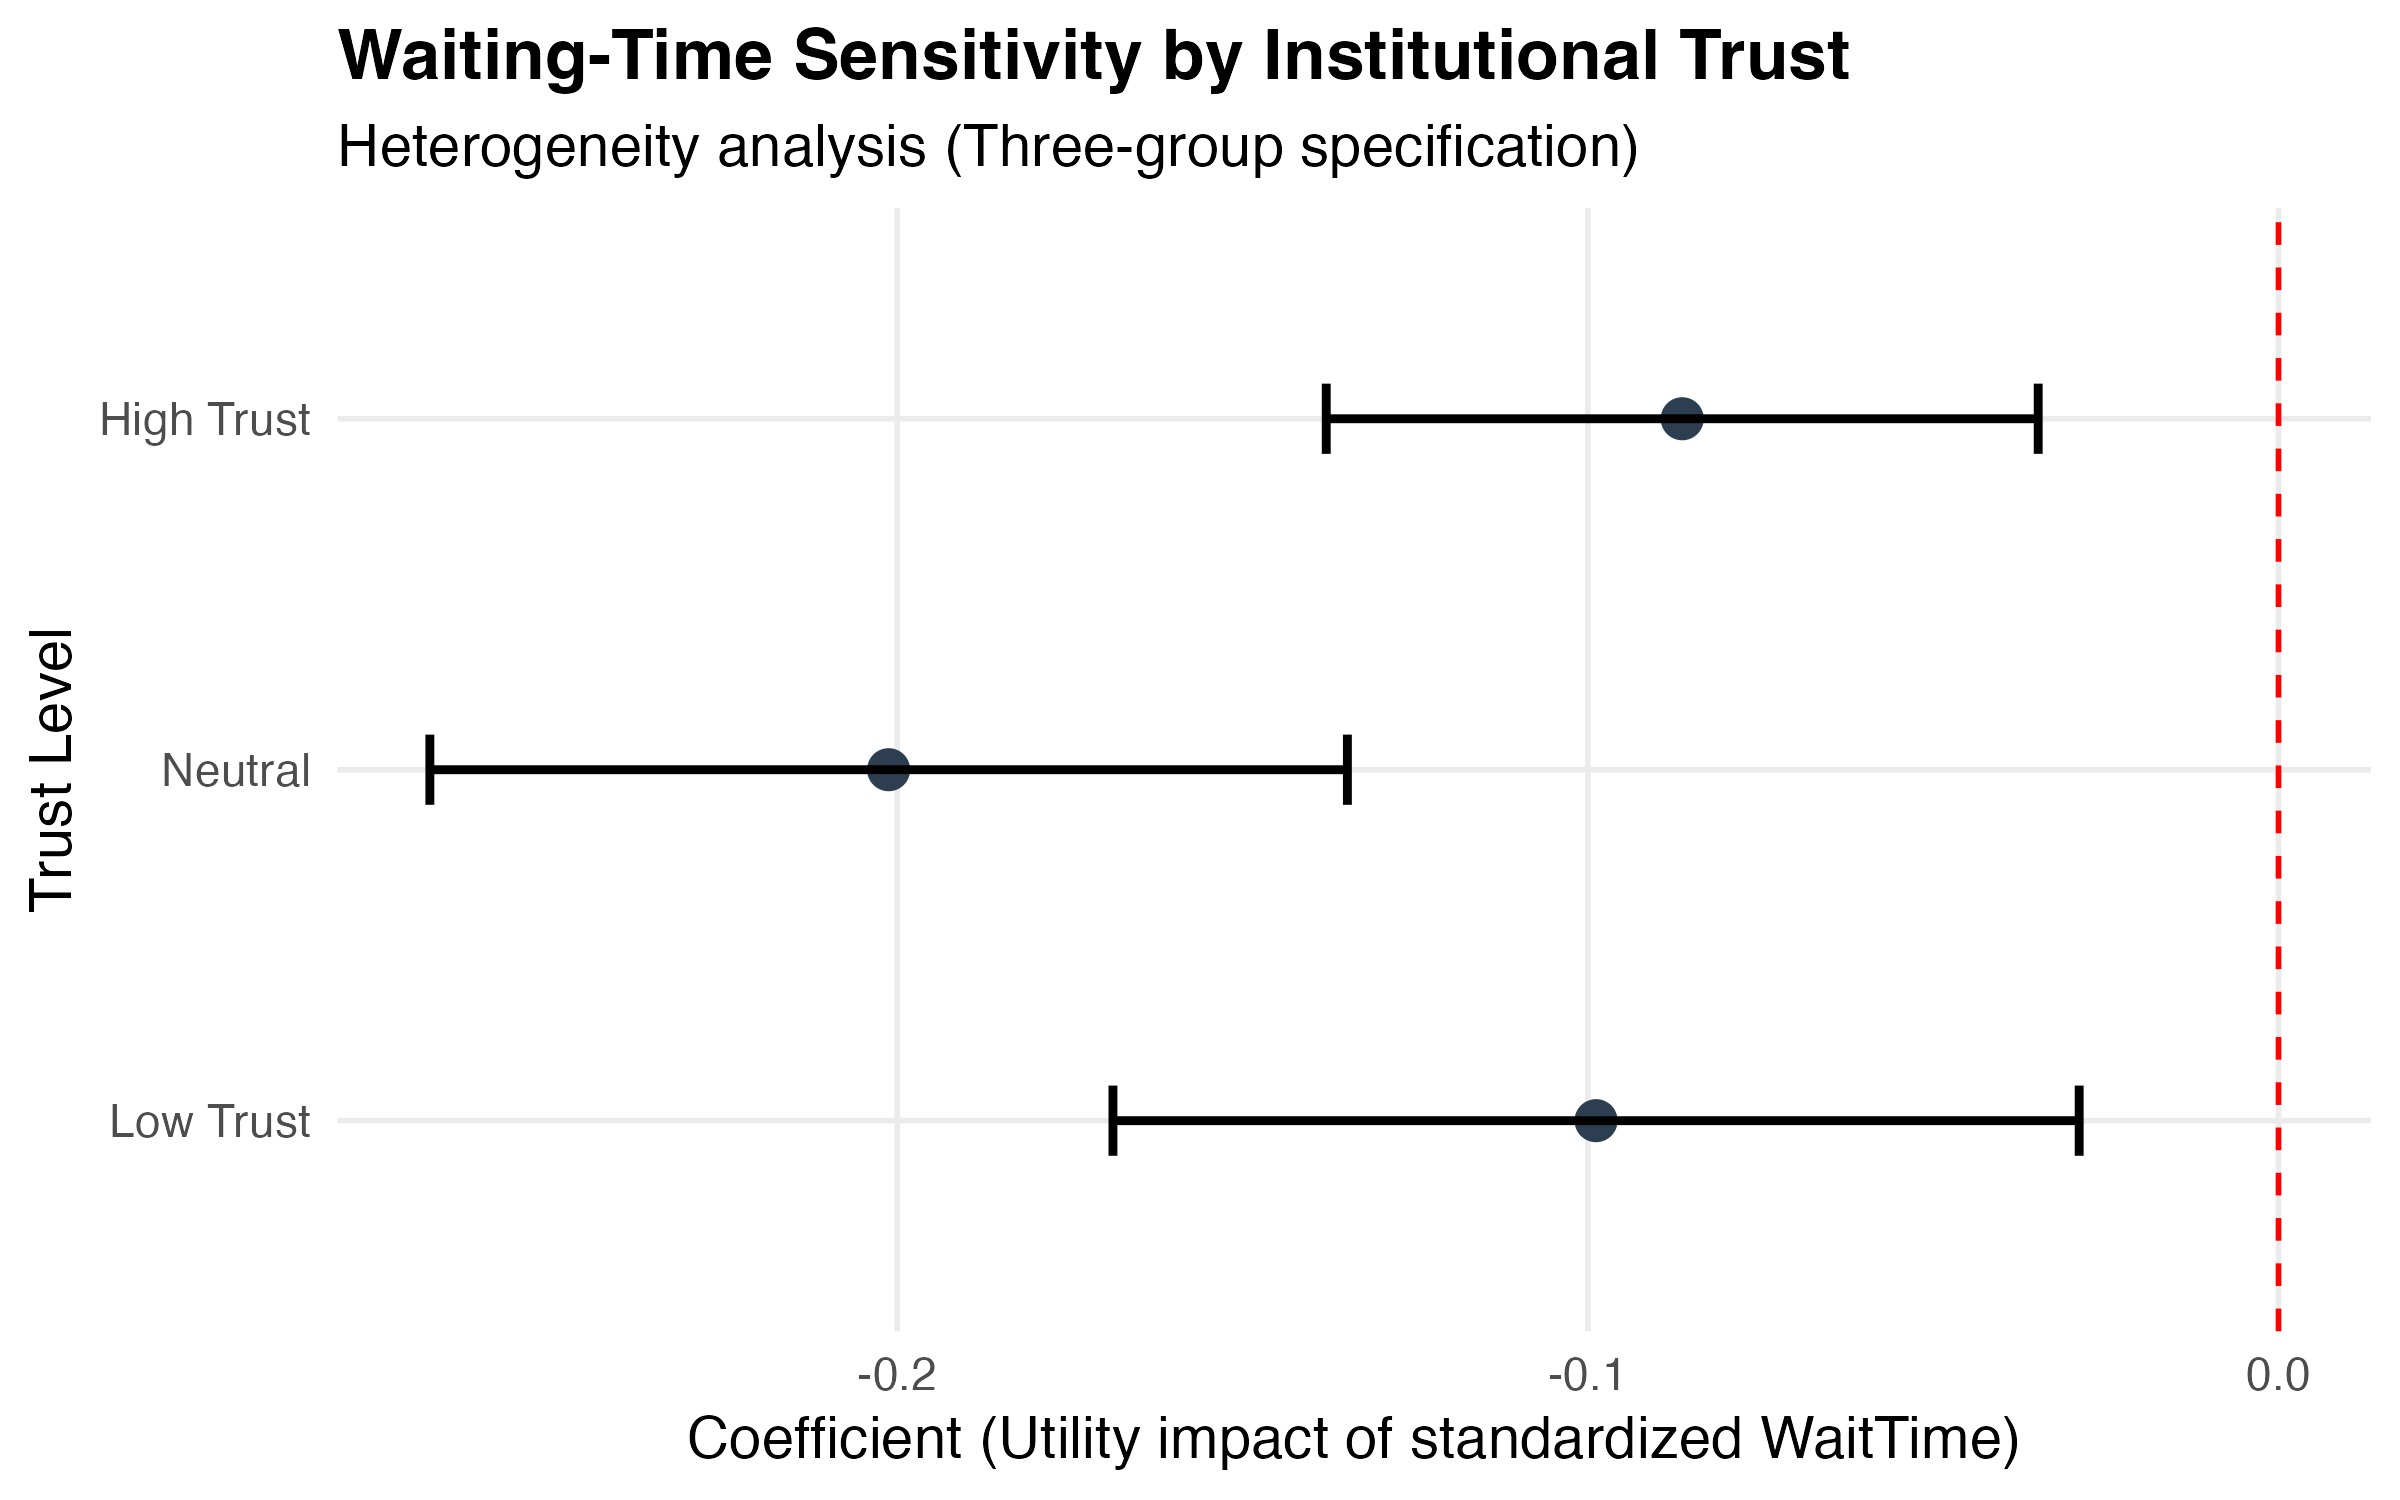
\includegraphics[width=\textwidth]{trust_heterogeneity_plot.png}
            \captionof{figure}{MWTA Comparison (RMB/month)}
        \end{column}
    \end{columns}
\end{frame}

% --- Slide 14: Results V: Shadow Price of Time (MWTA) ---
\begin{frame}{Results V: The Shadow Price of Vaccination Delay}
    \begin{itemize}
        \item \textbf{MWTA:} Marginal Willingness to Accept for a 1-month delay in protection.
        \item \textbf{Full Sample:} Mean MWTA = \textbf{45.2 RMB/month}.
        \item \textbf{Interpretation:} Individuals perceive a 1-month delay as equivalent to losing 45.2 RMB in utility (approx. \$6.3 USD).
    \end{itemize}
    \begin{center}
        \textbf{Takeaway: Administrative delays create a hidden, measurable welfare loss that varies by institutional trust.}
    \end{center}
\end{frame}

\section{Essay 3: Policy Simulation}

% --- Slide 15: Policy Simulation: Speed-up vs. Financial Compensation ---
\begin{frame}{Policy Simulation: Speed-up vs. Financial Compensation}
    \begin{center}
        \large \textbf{Is providing financial incentives more effective than reducing waiting times?}
    \end{center}

    \begin{columns}[c]
        \begin{column}{0.55\textwidth}
            \centering
            % --- Visual: Iso-acceptance Curves with Real Data ---
            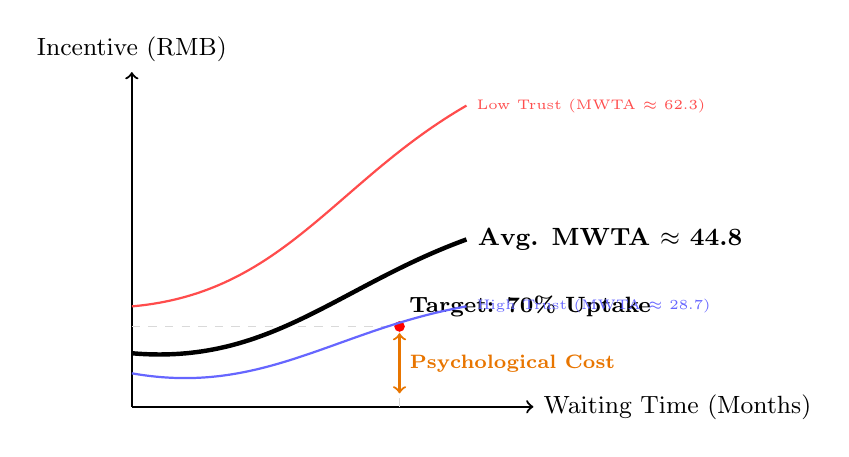
\begin{tikzpicture}[scale=0.85]
                % Axes
                \draw[thick, ->] (0,0) -- (6,0) node[right] {\small Waiting Time (Months)};
                \draw[thick, ->] (0,0) -- (0,5) node[above] {\small Incentive (RMB)};
                
                % Reference Grid
                \draw[dashed, gray!30] (0,1.2) -- (4,1.2);
                \draw[dashed, gray!30] (4,0) -- (4,1.2);
                
                % Data Points
                \filldraw[red] (4,1.2) circle (2pt) node[above right, black] {\footnotesize \textbf{Target: 70\% Uptake}};
                
                % Iso-acceptance Curves
                % High Trust (Flatter)
                \draw[blue!60, thick] (0,0.5) to[out=-10, in=190] (5,1.5) node[right] {\tiny High Trust (MWTA $\approx$ 28.7)};
                
                % Average (Main Results)
                \draw[black, ultra thick] (0,0.8) to[out=-5, in=200] (5,2.5) node[right] {\small \textbf{Avg. MWTA $\approx$ 44.8}};
                
                % Low Trust (Steeper)
                \draw[red!70, thick] (0,1.5) to[out=5, in=210] (5,4.5) node[right] {\tiny Low Trust (MWTA $\approx$ 62.3)};
                
                % Annotation for Trade-off
                \draw[<->, utdorange, thick] (4,0.2) -- (4,1.1) node[midway, right] {\scriptsize \textbf{Psychological Cost}};
            \end{tikzpicture}
        \end{column}

        \begin{column}{0.45\textwidth}
            \begin{block}{Welfare Implication (MWTA)}
                \small
                The \textbf{Marginal Willingness-to-Accept} for a 1-month delay:
                \begin{itemize}
                    \item \textbf{Full Sample}: \alert{44.8 RMB}
                    \item \textbf{Low Trust Group}: \alert{62.3 RMB}
                    \item \textbf{High Trust Group}: \alert{28.7 RMB}
                \end{itemize}
            \end{block}

            \vspace{0.3cm}
            \begin{itemize}
                \item \textbf{Policy Insight}: For the "Low Trust" group, reducing wait time is \textbf{2.1x} more effective than incentives.
                \item \textbf{Simulation}: $N=1,027$. Significant interaction ($p=0.021$) between delay and distrust.
            \end{itemize}
        \end{column}
    \end{columns}
\end{frame}

\section{Essay 3: Conclusion}

% --- Slide 16: The Social Planner's Decision Rule ---
\begin{frame}{The Social Planner's Decision Rule}
    \begin{itemize}
        \item \textbf{The Dilemma:} Speed up access ($C_{speed}$) vs. Compensate for delay ($C_{comp}$).
        \item \textbf{Efficiency Rule:} Invest in speed-up if the cost per month saved is lower than the shadow price (MWTA).
    \end{itemize}
    \begin{block}{Decision Framework}
        \centering
        \textbf{Operational Cost $\le$ MWTA} $\rightarrow$ \textbf{Prioritize Speed-Up} \\
        \textbf{Operational Cost $>$ MWTA} $\rightarrow$ \textbf{Prioritize Compensation}
    \end{block}
\end{frame}

% --- Slide 17: Equity-Sensitive Resource Allocation ---
\begin{frame}{Equity-Sensitive Resource Allocation}
    \begin{itemize}
        \item \textbf{The Rule:} Prioritize speed-up for Group $g$ if:
            \[ \text{Operational Cost} \le \omega_g \times MWTA_g \]
        \item \textbf{$\omega_g$}: Equity weight for vulnerable or high-burden groups.
        \item \textbf{Targeting:} High-burden groups (e.g., low-trust, low-income) have higher MWTA, making speed-up investments more valuable for them.
    \end{itemize}
\end{frame}

% --- Slide 18: Simulation Results: The Break-Even Point ---
\begin{frame}{Simulation: The 5.5-Month Threshold}
    \begin{itemize}
        \item \textbf{Scenario:} Reducing 1 month of delay costs 150 RMB per person.
        \item \textbf{Threshold:} At a baseline delay of \textbf{5.5 months}, the marginal cost of speeding up equals the marginal benefit of compensation.
        \item \textbf{Policy Implication:} For long delays (>5.5 months), incentives might be more cost-effective than infrastructure expansion.
    \end{itemize}
\end{frame}

\section{Conclusion}

% --- Slide 19: Summary of Contributions ---
\begin{frame}{Summary of Contributions}
    \begin{enumerate}
        \item \textbf{Measurement}: Quantified the Behavioral Delay Multiplier (1.29) and the Shadow Price (44.8 RMB/month).
        \item \textbf{Theory}: Demonstrated that hyperbolic discounting is the superior model for health timing decisions.
        \item \textbf{Practice}: Developed an actionable, equity-sensitive decision framework for vaccine rollout optimization.
    \end{enumerate}
\end{frame}

% --- Slide 20: Limitations and Future Work ---
\begin{frame}{Limitations and Future Work}
    \begin{itemize}
        \item \textbf{Stated vs. Revealed Preference}: Need validation with actual vaccination records.
        \item \textbf{External Validity}: Results are specific to Wuhan; extension to other regions and cultures is necessary.
        \item \textbf{Supply Chain Integration}: Connecting behavioral parameters with real-world vaccine logistics.
    \end{itemize}
\end{frame}

% --- Slide 21: Final Thought ---
\begin{frame}[plain]
    \centering
    \Huge \color{utdgreen} \textbf{Thank You!} \\
    \vspace{1cm}
    \large Questions \& Comments?
\end{frame}

\end{document}
